% =====================================================================
%  Introduction to Deep Learning — Class 11
%  Topic (course plan): Deep Networks
%  Subtopics (course plan): Activation functions, Error Functions,
%                           BackProp, automatic differentiation
%  Sources (course plan): Bishop Chapters 6-8, Prince Chapters 5 and 7
%
%  Classes 5-10 settled WHAT to build.  This class is the first on HOW
%  to train it.  Class 6 already derived the three standard error
%  functions from maximum likelihood; that is recapped in one slide and
%  then extended, not repeated.
%
%  Figures: generated by src/build_all.py (one module per figure).
%  Notation: the fixed course convention (see _shared/NOTATION.md).
%
%  Compile:  xelatex main.tex   (run twice)
% =====================================================================
\documentclass[aspectratio=169, 11pt]{beamer}

\usetheme{metropoliscustom}

\usepackage{graphicx}
\DeclareGraphicsExtensions{.pdf,.png,.jpg}
\graphicspath{{figs/}{Class11_Activations_Errors_Backprop_AD/B_Recreated_Figures/figs/}}
\usepackage{amsmath, amssymb}
\usepackage{bm}
\usepackage{tikz}
\usetikzlibrary{arrows.meta, positioning, calc, decorations.pathreplacing,
                shapes.geometric}
\tcbuselibrary{skins}

\definecolor{shc}{HTML}{341651}
\definecolor{tealc}{HTML}{1C7293}
\definecolor{dpc}{HTML}{800000}
\definecolor{accc}{HTML}{B8860B}

% ---- theorem environments -------------------------------------------
\setbeamertemplate{theorems}[numbered]
\newtheorem{lemmax}[theorem]{Lemma}
\newtheorem{propx}[theorem]{Proposition}
\newtheorem{corx}[theorem]{Corollary}
\newtheorem{algox}[theorem]{Algorithm}

% ---- parallel strip: forward (left) vs backward (right) --------------
\newcommand{\fbpar}[2]{%
  \vfill
  {\scriptsize
  \begin{tcolorbox}[enhanced, sidebyside, sidebyside align=top,
                    lefthand ratio=0.485,
                    segmentation style={shc!35, line width=0.6pt},
                    colback=shc!5, colframe=shc!35, boxrule=0.5pt,
                    arc=1.2mm, left=1.6mm, right=1.6mm,
                    top=0.6mm, bottom=0.6mm,
                    before skip=0pt, after skip=0pt]
    {\color{shc}\textbf{FORWARD}}\hspace{0.55em}#1
  \tcblower
    {\color{dpc}\textbf{BACKWARD}}\hspace{0.55em}#2
  \end{tcolorbox}}%
  \vspace{0.35em}%
}

\newcommand{\bridge}[1]{%
  {\scriptsize\itshape\color{mcMuted} #1\par}\vspace{0.35em}}

\newcommand{\figsource}[1]{{\scriptsize\color{mcMuted} #1}}
\newcommand{\figcap}[2][0.90]{%
  \begin{center}\begin{minipage}{#1\textwidth}\centering
    {\scriptsize\color{mcMuted} #2}
  \end{minipage}\end{center}}

\newcommand{\unit}[4]{%
  \node[circle, draw=#3, fill=#3!6, line width=0.7pt,
        minimum size=10mm, inner sep=0pt] (#1) at #2 {};
  \begin{scope}
    \clip #2 circle (0.5);
    \draw[tealc, line width=1.1pt]
      ($#2+(-0.50,-0.26)$) -- ($#2+(0.02,-0.26)$) -- ($#2+(0.46,0.28)$);
  \end{scope}
  \node[font=\large, #3] at ($#2+(0,0.78)$) {#4};
}
\newcommand{\plainunit}[4]{%
  \node[circle, draw=#3, fill=black!4, line width=0.7pt,
        minimum size=10mm, inner sep=0pt, font=\small] (#1) at #2 {#4};
}

% =====================================================================
\title{Deep Networks}
\subtitle{Activation Functions, Error Functions, Backpropagation and
          Automatic Differentiation}
\author{Introduction to Deep Learning \ \textperiodcentered\ Class 11}
\institute{}
\date{}

\footleft{Introduction to Deep Learning}
\footright{Backpropagation}
\titlelogos{}

\begin{document}

\maketitle

\begin{frame}{Outline}
  \tableofcontents
\end{frame}

% =====================================================================
\section{From What to How}
% =====================================================================

\begin{frame}{Notation used throughout this course}
  \vspace{0.2em}
  {\footnotesize
  \renewcommand{\arraystretch}{1.22}
  \begin{columns}[T, onlytextwidth]
    \begin{column}{0.49\textwidth}
      \begin{tabular}{@{}l@{\hspace{1.5em}}l@{}}
        $\mathbf{x}$, $y$, $\hat y$ & input, target, prediction\\
        $a^{(l)}_j$ & pre-activation, layer $l$\\
        $z^{(l)}_j = h(a^{(l)}_j)$ & activation\\
        $w^{(l)}_{ji}$ & weight into unit $j$ from unit $i$\\
        $h(\cdot)$, $h'(\cdot)$ & activation and its derivative\\
        $E(\mathbf{w})$, $E_n$ & total and per-example error\\
      \end{tabular}
    \end{column}
    \begin{column}{0.49\textwidth}
      \begin{tabular}{@{}l@{\hspace{1.5em}}l@{}}
        $\delta^{(l)}_j$ & $\partial E_n/\partial a^{(l)}_j$ \\
        $L$, $M$, $W$ & depth, width, parameter count\\
        $\mathbf{J}$ & Jacobian $\partial\hat{\mathbf{y}}/\partial\mathbf{x}$\\
        $\eta$ & learning rate\\
        $\dot v$, $\bar v$ & tangent, adjoint (\S5)\\
        $\odot$ & element-wise product\\
      \end{tabular}
    \end{column}
  \end{columns}}
  \vfill
  \begin{redhighlight}
    {\footnotesize The one new symbol is $\delta^{(l)}_j$, the
    \alert{error} at a unit. Everything in \S4 is a rule for computing
    it.}
  \end{redhighlight}
\end{frame}

\begin{frame}{Six lectures of \emph{what}; now \emph{how}}
  \vspace{0.2em}
  \begin{itemize}\setlength{\itemsep}{4pt}
    \item Classes 5--6: a network is regression on \alert{learned
          features}, and the error function follows from a
          \alert{distribution} over the output
    \item Classes 7--10: depth composes, universality holds, and
          \alert{depth is exponentially more efficient} than width
    \item Every one of those results is about the \alert{existence} of
          good weights
  \end{itemize}
  \vspace{0.4em}
  \begin{redhighlight}
    Training needs $\nabla E(\mathbf{w})$ --- one number for each of
    $W$ parameters, at every step. \alert{Getting it is today.}
  \end{redhighlight}
\end{frame}

\begin{frame}{Four questions}
  \vspace{0.05em}
  \centering
  \renewcommand{\arraystretch}{1.35}
  {\small
  \begin{tabular}{p{0.05\textwidth} p{0.44\textwidth}
                  p{0.38\textwidth}}
    & \textbf{Question} & \textbf{Where}\\
    \hline
    1 & Which $h$ should a hidden unit use, and why does it matter
        for \emph{training}?
      & \S2\\
    2 & Which error functions exist beyond the three from Class 6?
      & \S3\\
    3 & How do we get all $W$ derivatives at once?
      & \S4\\
    4 & Is backpropagation a special trick, or an instance of
        something general?
      & \S5\\
    \hline
  \end{tabular}}
  \vspace{0.4em}

  {\small The short answers: choose $h$ for its \alert{derivative};
  choose $E$ for the \alert{distribution}; get the gradient by the
  \alert{chain rule on a graph}; and that rule is
  \alert{reverse-mode automatic differentiation}.}
\end{frame}

% =====================================================================
\section{Activation Functions}
% =====================================================================

\begin{frame}{What the activation is for}
  \bridge{We have used ReLU without ever asking what the alternatives
  cost. Training is what settles the question.}
  \vspace{0.3em}
  \[
    a^{(l)}_j = \sum_i w^{(l)}_{ji} z^{(l-1)}_i + b^{(l)}_j,
    \qquad
    z^{(l)}_j = h\big(a^{(l)}_j\big)
  \]
  \vfill
  {\small
  \begin{itemize}\setlength{\itemsep}{4pt}
    \item Without $h$ the whole network collapses to one affine map
          (Class 5)
    \item Any non-polynomial $h$ gives universality (Class 9) --- so
          \alert{expressivity does not choose $h$ for us}
    \item What does choose it: the \alert{derivative} $h'$, because
          that is the factor every layer contributes to the gradient
  \end{itemize}}
  \fbpar{$h$ decides what the layer \emph{computes}}
        {$h'$ decides what the layer \emph{transmits}}
\end{frame}

\begin{frame}{The activation zoo: the rectifier family}
  \vspace{-0.5em}
  \begin{center}
    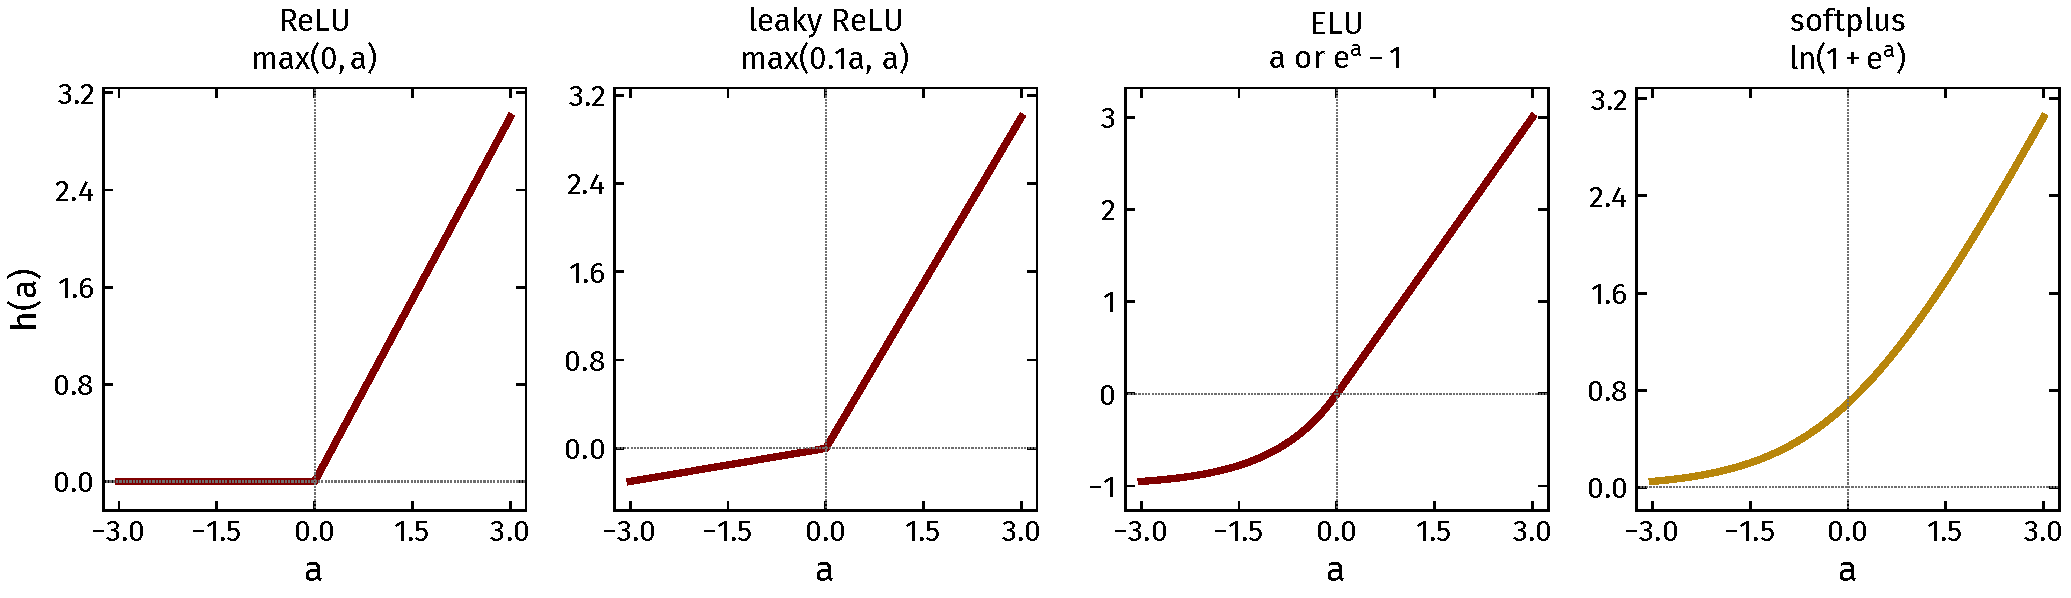
\includegraphics[width=0.99\linewidth]{activation_zoo_a}
  \end{center}
  \vspace{-0.55em}
  \figcap[0.96]{ReLU and the three ways of softening its corner --- all
  unbounded above, which is the property that matters.}
\end{frame}

\begin{frame}{The activation zoo: smooth and saturating}
  \vspace{-0.5em}
  \begin{center}
    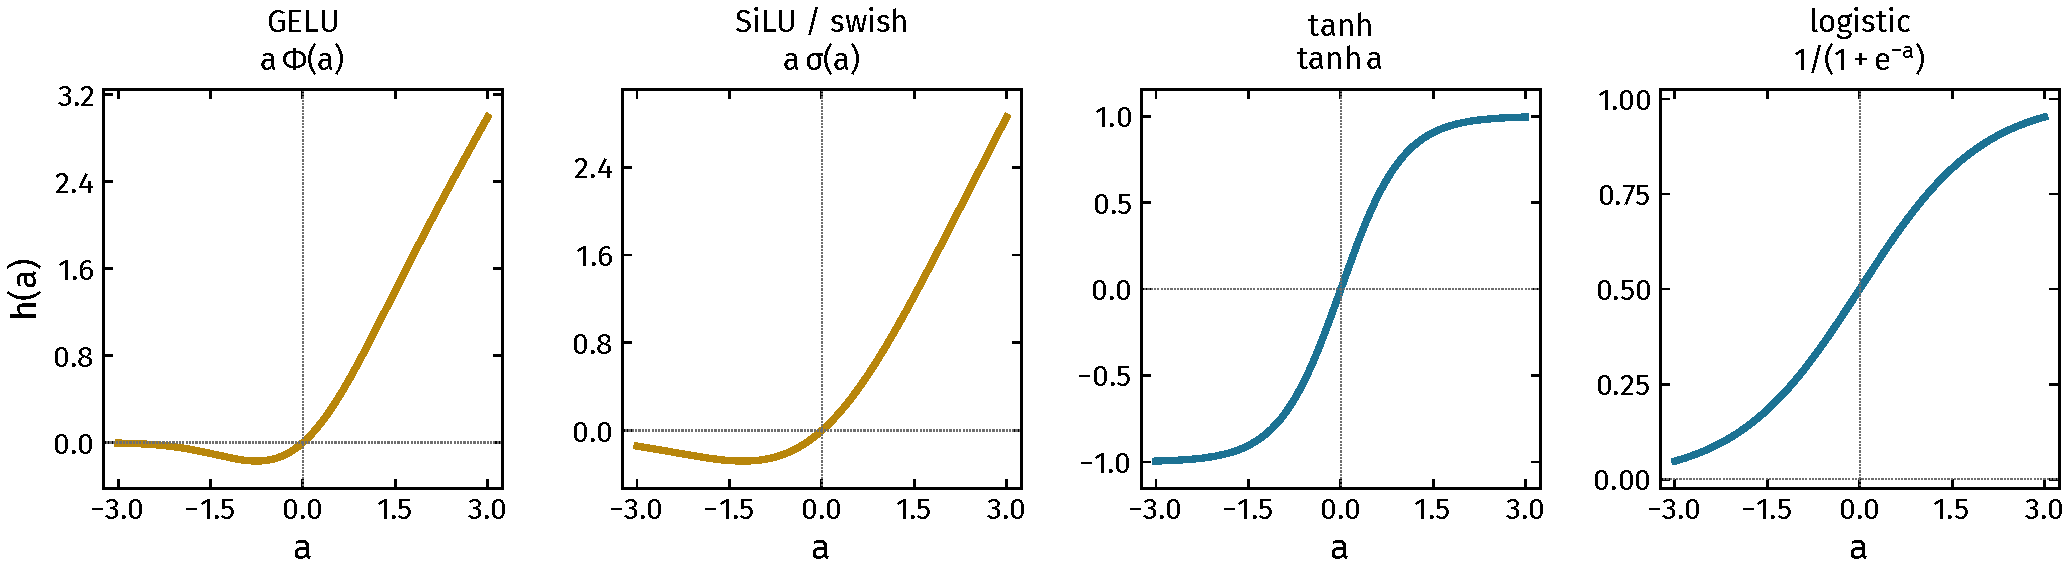
\includegraphics[width=0.99\linewidth]{activation_zoo_b}
  \end{center}
  \vspace{-0.55em}
  \figcap[0.96]{Top: the two modern smooth defaults. Bottom: the
  historical saturating pair, bounded above and below.}
\end{frame}

\begin{frame}{Differentiated: the rectifier family}
  \vspace{-0.5em}
  \begin{center}
    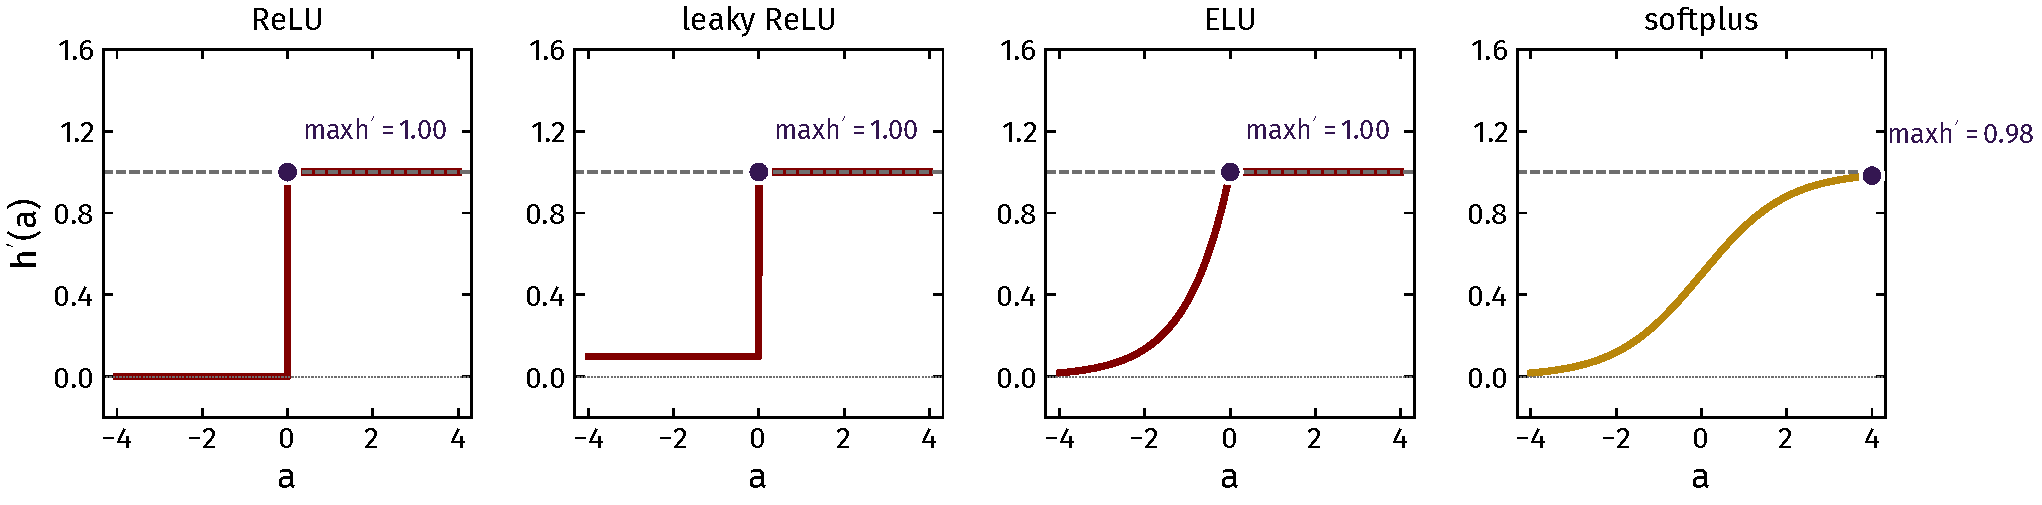
\includegraphics[width=0.99\linewidth]{activation_derivatives_a}
  \end{center}
  \vspace{-0.55em}
  \figcap[0.97]{The marked point is $\max h'$: the \alert{best} factor a
  layer can contribute to the backward pass. All four reach $1$, so the
  gradient can pass undiminished.}
\end{frame}

\begin{frame}{Differentiated: smooth and saturating}
  \vspace{-0.5em}
  \begin{center}
    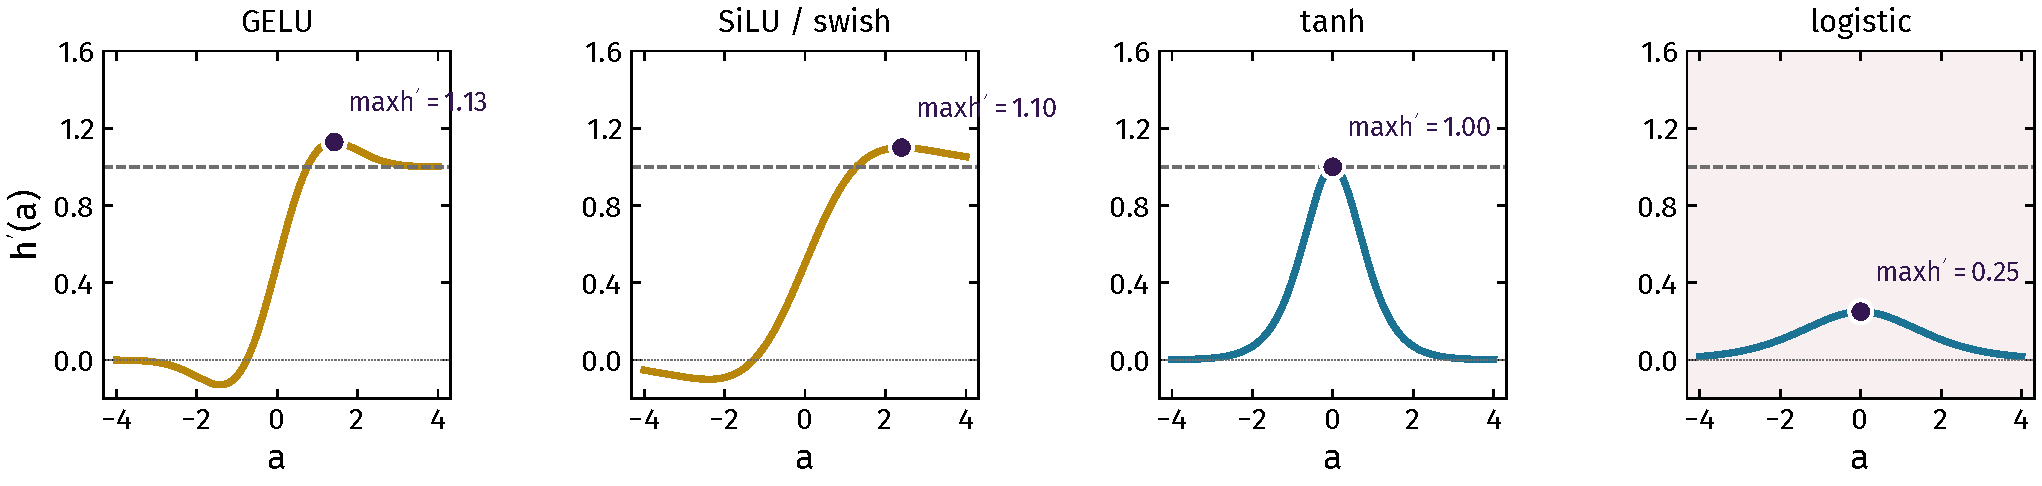
\includegraphics[width=0.99\linewidth]{activation_derivatives_b}
  \end{center}
  \vspace{-0.55em}
  \figcap[0.97]{The logistic caps $\max h'$ at $0.25$, so $L$ layers
  multiply the gradient by at most $4^{-L}$ --- whatever the weights
  are.}
\end{frame}

\begin{frame}{Why the logistic sigmoid fails at depth}
  \vspace{0.2em}
  \begin{propx}[The sigmoid derivative is bounded by $1/4$]
    {\small For all $a$, $\ \sigma'(a)=\sigma(a)\big(1-\sigma(a)\big)
    \leq \tfrac14$, with equality only at $a=0$.}
  \end{propx}
  \vspace{0.2em}
  {\footnotesize
  \begin{itemize}\setlength{\itemsep}{2pt}
    \item \focus{1}{Write $u=\sigma(a)\in(0,1)$, so
          $\sigma'=u(1-u)$}
    \item \focus{2}{$u(1-u)=\tfrac14-\big(u-\tfrac12\big)^{2}$, a
          downward parabola in $u$}
    \item \focus{3}{Hence $u(1-u)\leq\tfrac14$, with equality iff
          $u=\tfrac12$, i.e.\ $a=0$ \hfill $\square$}
  \end{itemize}}
  \vspace{0.2em}
  \begin{corx}[Sigmoid networks vanish]
    {\small Crossing $L$ sigmoid layers multiplies the backpropagated
    signal by at most $4^{-L}$. At $L=10$ that is under $10^{-6}$
    before any weight is taken into account.}
  \end{corx}
\end{frame}

\begin{frame}{Saturation, drawn}
  \begin{center}
    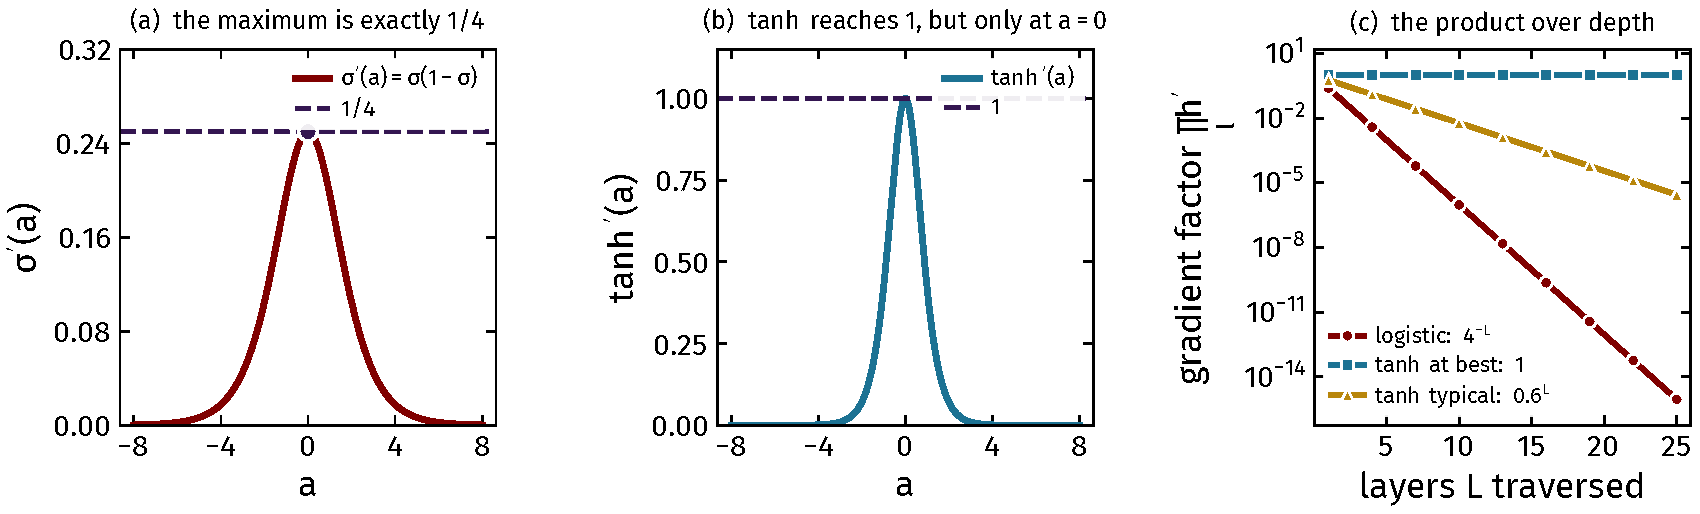
\includegraphics[height=0.485\textheight]{saturation_bound}
  \end{center}
  \figcap[0.96]{(a) $\sigma'$ peaks at exactly $1/4$. (b) $\tanh'$
  reaches $1$, but only at the origin --- which is why $\tanh$ was
  preferred to the logistic for decades. (c) the product over depth:
  $4^{-L}$ is hopeless, and even a typical $\tanh$ factor of $0.6$
  costs four orders of magnitude by $L=20$.}
\end{frame}

\begin{frame}{The rectifier's own failure mode}
  \vspace{0.2em}
  \begin{propx}[Dead units are permanent]
    {\small If a ReLU unit has $a_j(\mathbf{x}_n)\leq 0$ for
    \alert{every} training input, then $z_j\equiv 0$ and
    $\partial E/\partial w_{ji}=0$ for all $i$. No gradient step can
    change its weights, so it stays dead for the rest of training.}
  \end{propx}
  \vspace{0.2em}
  {\footnotesize
  \emph{Proof.} $\partial E_n/\partial w_{ji}
  = \delta_j z_i$ and $\delta_j = h'(a_j)\sum_k w_{kj}\delta_k$.
  For $a_j<0$, $h'(a_j)=0$, so $\delta_j=0$ for every $n$, hence every
  derivative into the unit vanishes. \hfill$\square$}
  \vspace{0.3em}
  {\small
  \begin{itemize}\setlength{\itemsep}{3pt}
    \item ReLU trades \alert{saturation on one side} for
          \alert{exact zero on the other}
    \item Leaky ReLU, ELU, GELU and SiLU all keep a small non-zero
          slope for $a<0$ for exactly this reason
  \end{itemize}}
\end{frame}

\begin{frame}{A unit switching off, drawn}
  \begin{center}
    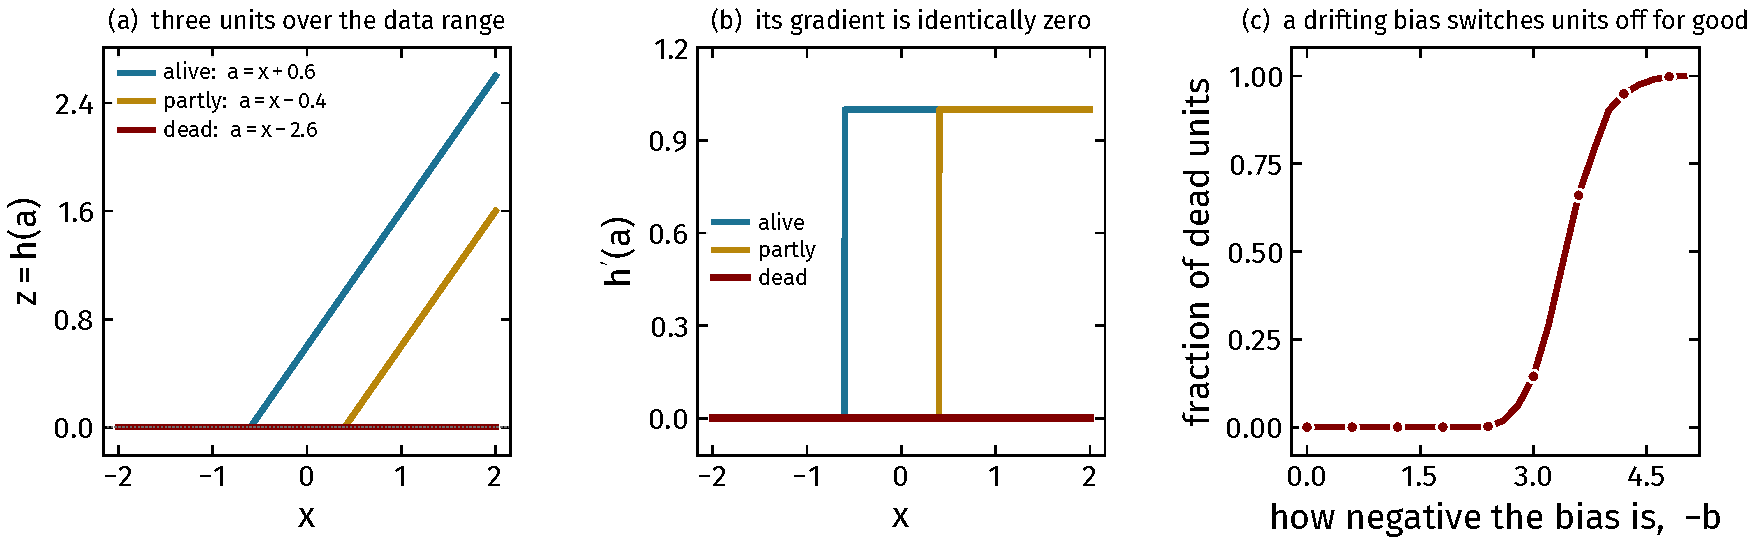
\includegraphics[height=0.485\textheight]{dying_relu}
  \end{center}
  \figcap[0.96]{(a) three units over the data range: one active
  throughout, one active on part of it, one never active. (b) their
  derivatives --- the dead unit's is identically zero. (c) as gradient
  descent drives a bias negative, the fraction of permanently dead
  units climbs sharply.}
\end{frame}

\begin{frame}{Choosing an activation}
  \vspace{0.05em}
  \centering
  \renewcommand{\arraystretch}{1.25}
  {\footnotesize
  \begin{tabular}{p{0.17\textwidth} p{0.20\textwidth}
                  p{0.24\textwidth} p{0.28\textwidth}}
    \textbf{Activation} & \textbf{$h'$ range} & \textbf{Strength}
      & \textbf{Weakness}\\
    \hline
    logistic & $(0,\tfrac14]$ & bounded output
      & vanishes at depth\\
    $\tanh$ & $(0,1]$ & zero-centred
      & still saturates\\
    ReLU & $\{0,1\}$ & no saturation for $a>0$, cheap
      & dead units, not differentiable at $0$\\
    leaky ReLU & $\{s,1\}$ & never exactly zero
      & one more hyperparameter\\
    ELU & $(0,1]$ & smooth, saturates below
      & exponential to evaluate\\
    GELU / SiLU & $(-0.1,1.1)$ & smooth, the current default
      & no simple intuition\\
    \hline
  \end{tabular}}
  \vspace{0.05em}
  {\small Read the second column first: an activation is chosen for the
  \alert{gradient it lets through}, not the shape it draws.}
\end{frame}

% =====================================================================
\section{Error Functions, Revisited}
% =====================================================================

\begin{frame}{What Class 6 established}
  \bridge{The output end of the network was settled in Class 6. One
  slide to recall it, then the cases it did not cover.}
  \vspace{0.3em}
  \centering
  \renewcommand{\arraystretch}{1.3}
  {\small
  \begin{tabular}{p{0.17\textwidth} p{0.17\textwidth}
                  p{0.22\textwidth} p{0.28\textwidth}}
    \textbf{Task} & \textbf{Distribution} &
    \textbf{Output activation} & \textbf{Error}\\
    \hline
    Regression & Gaussian & identity & sum of squares\\
    Binary & Bernoulli & sigmoid & binary cross-entropy\\
    Multi-class & categorical & softmax & cross-entropy\\
    \hline
  \end{tabular}}
  \vspace{0.6em}

  {\small Choose the distribution; the output activation and the error
  function are then \alert{determined}. And in all three cases
  $\partial E_n/\partial a_k = \hat y_k - y_k$.}
  \vspace{0.3em}

  {\small That last fact looked like a coincidence three times over.
  It is not.}
\end{frame}

\begin{frame}{Why the output gradient is always $\hat y - y$}
  \vspace{0.05em}
  \begin{theorem}[Canonical link]
    {\small Let the output distribution be an exponential family
    $p(y\mid\theta)=\exp\{\theta y - A(\theta) + c(y)\}$, let the
    network's output pre-activation be its natural parameter,
    $\theta = a$, and let $E_n=-\ln p(y_n\mid a_n)$. Then
    \[
      \frac{\partial E_n}{\partial a_n} \;=\; \hat y_n - y_n,
      \qquad \hat y_n = A'(a_n) = \mathbb{E}[y\mid a_n].
    \]}
  \end{theorem}
  \vspace{-0.05em}
  {\footnotesize
  \begin{itemize}\setlength{\itemsep}{0pt}
    \item \focus{1}{$E_n = -\theta y_n + A(\theta) - c(y_n)$ with
          $\theta=a_n$}
    \item \focus{2}{Differentiate: $\partial E_n/\partial a_n
          = -y_n + A'(a_n)$}
    \item \focus{3}{For an exponential family $A'(\theta)$ is the
          mean --- exactly what the output activation produces
          \hfill $\square$}
    \item \focus{4}{Gaussian gives the identity, Bernoulli the
          sigmoid, categorical the softmax --- \alert{the three cases
          of Class 6 are one theorem}}
  \end{itemize}}
\end{frame}

\begin{frame}{Why this matters for training}
  \vspace{0.3em}
  {\small
  \begin{itemize}\setlength{\itemsep}{5pt}
    \item The output layer contributes \alert{no $h'$ factor at all}:
          the $A''$ from the link and the $1/\mathrm{var}$ from the
          error cancel
    \item Mismatch the pair --- squared error on a sigmoid output ---
          and the factor comes back as $\sigma'(a)$, which we now know
          is at most $1/4$ (Class 6, and \S2 today)
    \item So the canonical pairing is not aesthetics: it removes one
          source of vanishing gradient at the point where the signal
          enters the network
  \end{itemize}}
  \vspace{0.4em}
  \begin{redhighlight}
    {\small Backpropagation starts with $\delta^{(L+1)}=\hat y - y$.
    Everything in \S4 is about propagating that first $\delta$
    downwards.}
  \end{redhighlight}
\end{frame}

\begin{frame}{When one number per input is not enough}
  \bridge{The three standard cases all assume the noise is the same
  everywhere. Two common situations where it is not.}
  \begin{center}
    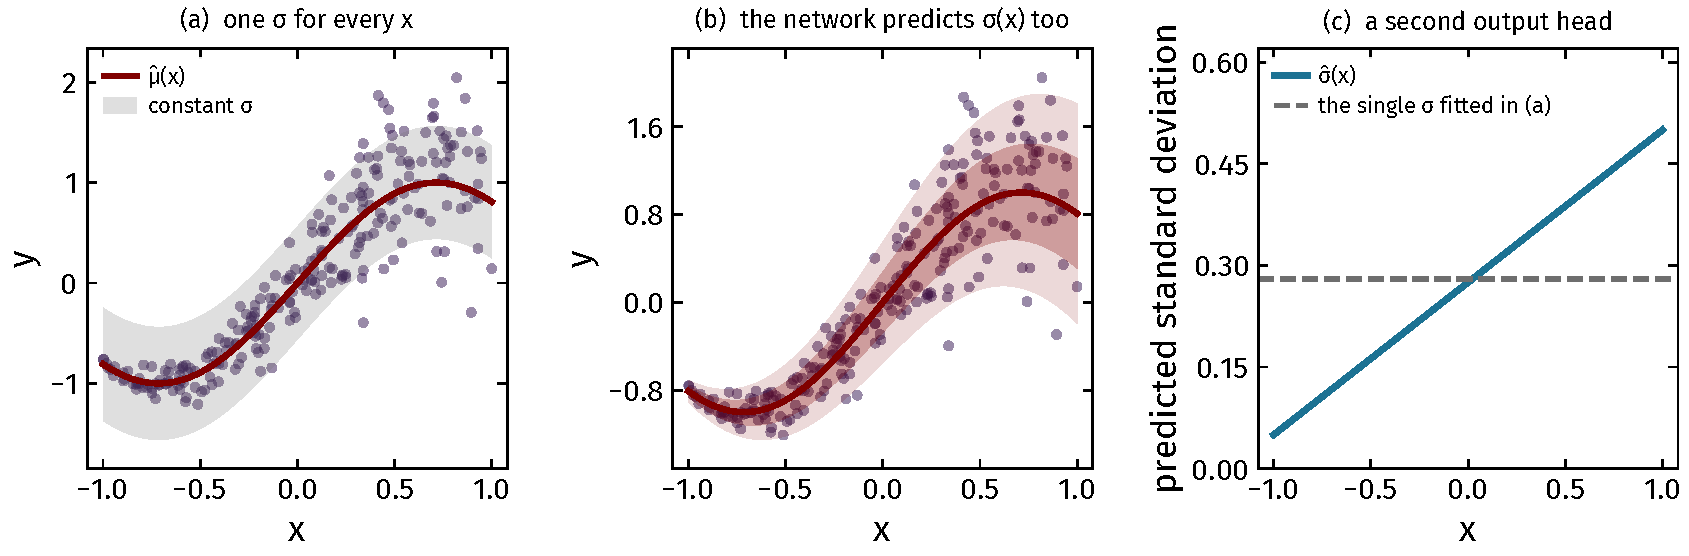
\includegraphics[height=0.41\textheight]{heteroscedastic}
  \end{center}
  \figcap[0.96]{(a) a single fitted $\sigma$ is too wide on the left and
  too narrow on the right. (b) giving the network a second output head
  for $\sigma(x)$ fixes it. (c) the predicted standard deviation. The
  error function becomes
  $E_n=\tfrac{(y_n-\hat\mu_n)^2}{2\hat\sigma_n^{2}}+\ln\hat\sigma_n$,
  with $\hat\sigma=\exp(\cdot)$ to keep it positive.}
\end{frame}

\begin{frame}{When the target is genuinely multi-valued}
  \begin{center}
    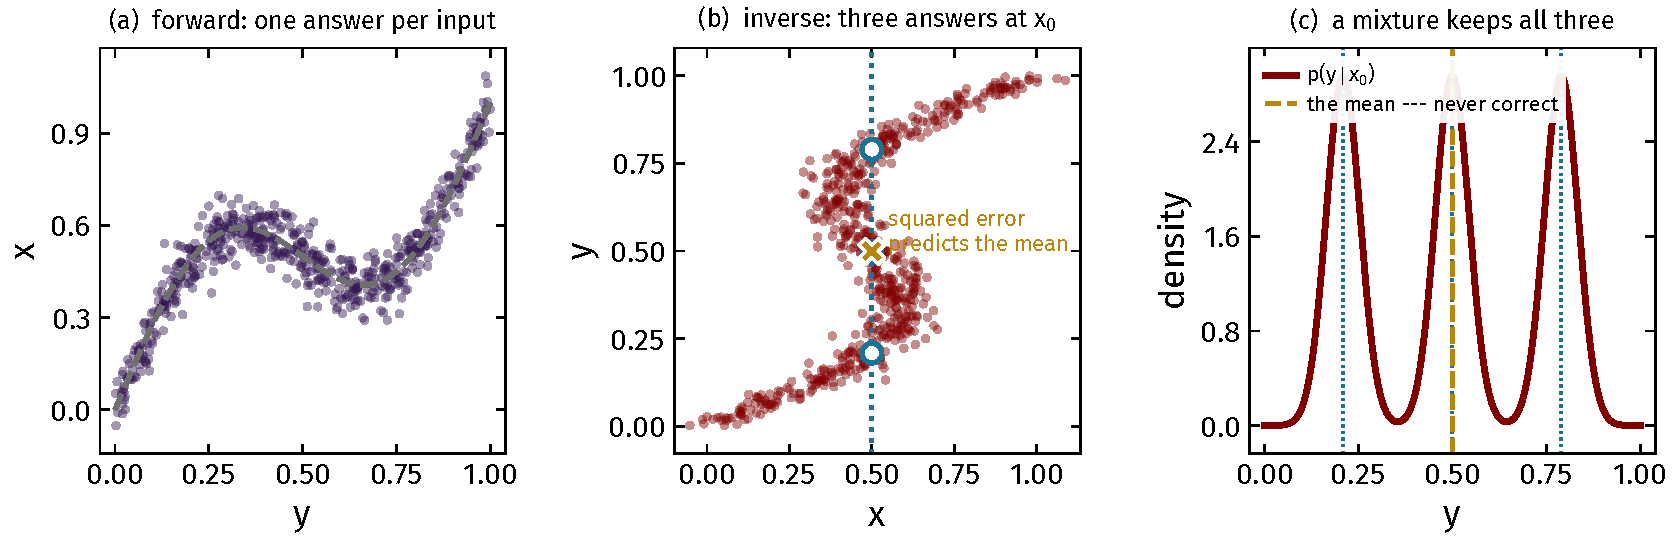
\includegraphics[height=0.44\textheight]{mixture_density}
  \end{center}
  \figcap[0.96]{(a) a forward map with one answer per input. (b) read
  backwards it has three, and a network trained on squared error
  predicts their \emph{average} --- a value that is never a correct
  answer. (c) a \alert{mixture density network} predicts $\pi_k$,
  $\mu_k$, $\sigma_k$ instead, and keeps all three modes.}
  \vspace{-0.1em}
  {\footnotesize
  \begin{itemize}\setlength{\itemsep}{0pt}
    \item $p(y\mid\mathbf{x})=\sum_k \pi_k(\mathbf{x})\,
          \mathcal{N}\big(y\mid\mu_k(\mathbf{x}),
          \sigma_k^{2}(\mathbf{x})\big)$
          \hfill{\scriptsize Bishop \& Bishop, \S6.5}
  \end{itemize}}
\end{frame}

% =====================================================================
\section{Backpropagation}
% =====================================================================

\begin{frame}{The problem, stated}
  \bridge{We have an error function and an architecture. Gradient
  descent needs one number per parameter, and there are $W$ of them.}
  \vspace{0.3em}
  \[
    \mathbf{w} \leftarrow \mathbf{w} - \eta\,\nabla E(\mathbf{w}),
    \qquad
    \nabla E = \Big(\frac{\partial E}{\partial w_1},\dots,
    \frac{\partial E}{\partial w_W}\Big)^{\!\top}
  \]
  \vfill
  {\small
  \begin{itemize}\setlength{\itemsep}{4pt}
    \item A modern network has $W$ in the millions or billions, and the
          gradient is needed \alert{every step}
    \item Two obvious approaches --- perturb each weight, or
          differentiate symbolically --- both fail, for different
          reasons
    \item The way out is that $E$ is a \alert{composition}, and a
          composition can be differentiated once and reused
  \end{itemize}}
\end{frame}

\begin{frame}{Why not just perturb each weight?}
  \begin{center}
    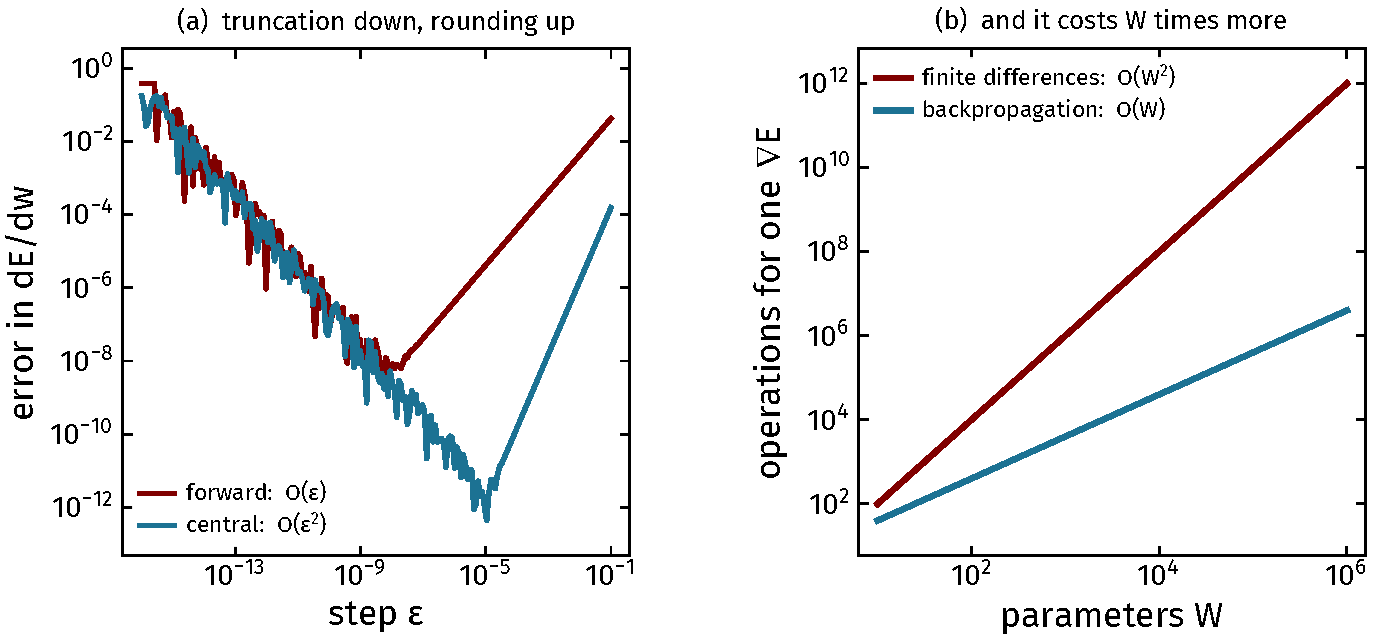
\includegraphics[height=0.445\textheight]{diff_methods}
  \end{center}
  \figcap[0.96]{(a) a finite difference has two competing errors:
  truncation falls with the step, rounding rises, and the best
  attainable accuracy is around $10^{-8}$ even for central differences.
  (b) worse, each of the $W$ derivatives needs its own forward pass, so
  one gradient costs $O(W^{2})$ operations against
  backpropagation's $O(W)$.}
  \vspace{-0.1em}
  {\footnotesize
  \begin{itemize}\setlength{\itemsep}{0pt}
    \item Still useful for \alert{checking} an implementation on a
          small network --- and only for that
  \end{itemize}}
\end{frame}

\begin{frame}{The one idea}
  \vspace{0.0em}
  {\small A weight $w^{(l)}_{ji}$ affects $E$ \alert{only through} the
  pre-activation $a^{(l)}_j$ it feeds. So the chain rule splits every
  derivative into two factors:}
  \vspace{0.05em}
  \[
    \frac{\partial E_n}{\partial w^{(l)}_{ji}}
    \;=\;
    \underbrace{\frac{\partial E_n}{\partial a^{(l)}_j}}_{\textstyle
      \delta^{(l)}_j}
    \;\cdot\;
    \underbrace{\frac{\partial a^{(l)}_j}{\partial w^{(l)}_{ji}}}_{
      \textstyle z^{(l-1)}_i}
    \;=\; \delta^{(l)}_j\, z^{(l-1)}_i
    \tag{B\&B 8.3--8.5}
  \]
  \vfill
  {\small
  \begin{itemize}\setlength{\itemsep}{0pt}
    \item $z^{(l-1)}_i$ is already known --- computed on the way
          \alert{up}
    \item So the problem reduces to the $\delta^{(l)}_j$: one per
          \emph{unit} rather than one per \emph{weight}, and they
          satisfy a recursion
  \end{itemize}}
  \fbpar{store every $z^{(l)}$}
        {compute every $\delta^{(l)}$, then multiply}
\end{frame}

\begin{frame}{The backpropagation equations}
  \vspace{0.05em}
  \begin{theorem}[Backpropagation]
    {\small For a feed-forward network with error $E_n$ and
    differentiable activation $h$,
    \[
      \delta^{(L+1)} = \hat{\mathbf{y}}_n - \mathbf{y}_n,
      \qquad
      \delta^{(l)}_j = h'\big(a^{(l)}_j\big)
      \sum_k w^{(l+1)}_{kj}\,\delta^{(l+1)}_k,
      \qquad
      \frac{\partial E_n}{\partial w^{(l)}_{ji}}
      = \delta^{(l)}_j z^{(l-1)}_i .
    \]}
  \end{theorem}
  \vspace{-0.05em}
  {\footnotesize
  \begin{itemize}\setlength{\itemsep}{0pt}
    \item \focus{1}{$a^{(l)}_j$ reaches $E_n$ only through the units
          $k$ it feeds:
          $\delta^{(l)}_j=\sum_k \frac{\partial E_n}{\partial
          a^{(l+1)}_k}\frac{\partial a^{(l+1)}_k}{\partial a^{(l)}_j}$}
    \item \focus{2}{The first factor is $\delta^{(l+1)}_k$ by
          definition}
    \item \focus{3}{For the second,
          $a^{(l+1)}_k=\sum_j w^{(l+1)}_{kj} h(a^{(l)}_j)$, so
          $\partial a^{(l+1)}_k/\partial a^{(l)}_j
          = w^{(l+1)}_{kj}h'(a^{(l)}_j)$}
    \item \focus{4}{Substituting and pulling $h'$ out of the sum gives
          the recursion; the top-layer value is the canonical-link
          theorem of \S3 \hfill $\square$}
  \end{itemize}}
\end{frame}

\begin{frame}{The algorithm}
  \vspace{0.2em}
  \begin{algox}[Backpropagation for one example]
    {\small
    \begin{enumerate}\setlength{\itemsep}{2pt}
      \item \textbf{Forward.} Set $\mathbf{z}^{(0)}=\mathbf{x}_n$ and
            for $l=1,\dots,L$ compute
            $\mathbf{a}^{(l)}=\mathbf{W}^{(l)}\mathbf{z}^{(l-1)}
            +\mathbf{b}^{(l)}$ and
            $\mathbf{z}^{(l)}=h(\mathbf{a}^{(l)})$. \alert{Store every
            $\mathbf{a}^{(l)}$ and $\mathbf{z}^{(l)}$.}
      \item \textbf{Output error.} $\bm\delta^{(L+1)}
            =\hat{\mathbf{y}}_n-\mathbf{y}_n$.
      \item \textbf{Backward.} For $l=L,\dots,1$,
            $\bm\delta^{(l)} = h'(\mathbf{a}^{(l)})\odot
            \big(\mathbf{W}^{(l+1)\top}\bm\delta^{(l+1)}\big)$.
      \item \textbf{Derivatives.}
            $\partial E_n/\partial\mathbf{W}^{(l)}
            = \bm\delta^{(l)}\mathbf{z}^{(l-1)\top}$ and
            $\partial E_n/\partial\mathbf{b}^{(l)}=\bm\delta^{(l)}$.
    \end{enumerate}}
  \end{algox}
  \vspace{0.2em}
  {\small Sum over $n$ for the full-batch gradient.}
\end{frame}

\begin{frame}{A worked pass, by hand}
  \centering
  \begin{tikzpicture}[>=Stealth, line width=0.8pt, font=\small,
      scale=0.665, transform shape]
    \plainunit{x}{(0,0)}{black!55}{$x$}
    \unit{h1}{(2.6,1.3)}{shc}{$z_1$}
    \unit{h2}{(2.6,-1.3)}{shc}{$z_2$}
    \plainunit{y}{(5.2,0)}{dpc}{$\hat y$}
    \draw[->, black!45] (x)--node[above,font=\scriptsize]{$w_{11}$}(h1);
    \draw[->, black!45] (x)--node[below,font=\scriptsize]{$w_{21}$}(h2);
    \draw[->, black!45] (h1)--node[above,font=\scriptsize]{$v_{1}$}(y);
    \draw[->, black!45] (h2)--node[below,font=\scriptsize]{$v_{2}$}(y);
    \draw[->, dpc, line width=1.4pt] (5.9,-0.55) -- (4.6,-0.55)
      node[midway, below, font=\scriptsize, dpc] {$\delta=\hat y-y$};
  \end{tikzpicture}
  \vspace{0.05em}
  {\footnotesize
  \begin{columns}[T, onlytextwidth]
    \begin{column}{0.47\textwidth}
      \textbf{Forward}
      \begin{align*}
        a_j &= w_{j1}x, \qquad z_j = h(a_j)\\
        a   &= v_1 z_1 + v_2 z_2, \quad \hat y = a
      \end{align*}
    \end{column}
    \begin{column}{0.50\textwidth}
      \textbf{Backward}
      \begin{align*}
        \delta &= \hat y - y\\
        \delta_j &= h'(a_j)\,v_j\,\delta\\
        \frac{\partial E}{\partial v_j} &= \delta\, z_j,
        \qquad
        \frac{\partial E}{\partial w_{j1}} = \delta_j\, x
      \end{align*}
    \end{column}
  \end{columns}}
  \vspace{0.05em}
  \figcap[0.94]{Four derivatives, one forward pass and one backward
  pass --- no derivative is ever computed twice.}
\end{frame}

\begin{frame}{What it costs}
  \vspace{0.2em}
  \begin{propx}[Backpropagation is $O(W)$]
    {\small For a network with $W$ weights, one forward pass costs
    $O(W)$ multiply--adds, and the backward pass costs another $O(W)$.
    The complete gradient therefore costs $O(W)$ --- a small constant
    times the cost of one forward evaluation.}
  \end{propx}
  \vspace{0.2em}
  {\footnotesize
  \emph{Proof.} Each weight is used exactly once in the forward pass
  (in the sum forming its target's pre-activation) and exactly once in
  the backward pass (in the sum forming its source's $\delta$). Every
  unit contributes one evaluation of $h$ and one of $h'$, and there are
  fewer units than weights. \hfill$\square$}
  \vspace{0.4em}
  {\small
  \begin{itemize}\setlength{\itemsep}{3pt}
    \item Compare $O(W^{2})$ for finite differences: at $W=10^{6}$ that
          is a factor of a million
    \item This single fact is why gradient-based training of large
          networks is possible at all
  \end{itemize}}
\end{frame}

\begin{frame}{The recursion has a price: vanishing and exploding}
  \bridge{The backward pass multiplies by $h'$ and by $\mathbf{W}^\top$
  once per layer. Repeated multiplication is unstable in both
  directions.}
  \vspace{0.2em}
  \begin{propx}[Gradient scaling across layers]
    {\small
    $\bm\delta^{(l)} = \big(\textstyle\prod_{m=l+1}^{L}
    \mathbf{D}^{(m)}\mathbf{W}^{(m)\top}\big)\bm\delta^{(L+1)}$ with
    $\mathbf{D}^{(m)}=\mathrm{diag}\,h'(\mathbf{a}^{(m)})$, so
    $\lVert\bm\delta^{(l)}\rVert
    \leq \prod_m \lVert\mathbf{W}^{(m)}\rVert\,
    \sup|h'| \cdot \lVert\bm\delta^{(L+1)}\rVert$: the bound is a
    \alert{product of $L-l$ factors} and is therefore exponential in
    depth unless those factors sit near $1$.}
  \end{propx}
  \vspace{0.4em}
  {\small
  \begin{itemize}\setlength{\itemsep}{3pt}
    \item Factor below $1$: the gradient \alert{vanishes} and early
          layers stop learning
    \item Factor above $1$: it \alert{explodes} and the step overshoots
    \item Fixes are Classes 12--15: careful initialisation,
          normalisation, residual connections, gradient clipping
  \end{itemize}}
\end{frame}

\begin{frame}{Measured, over twenty layers}
  \begin{center}
    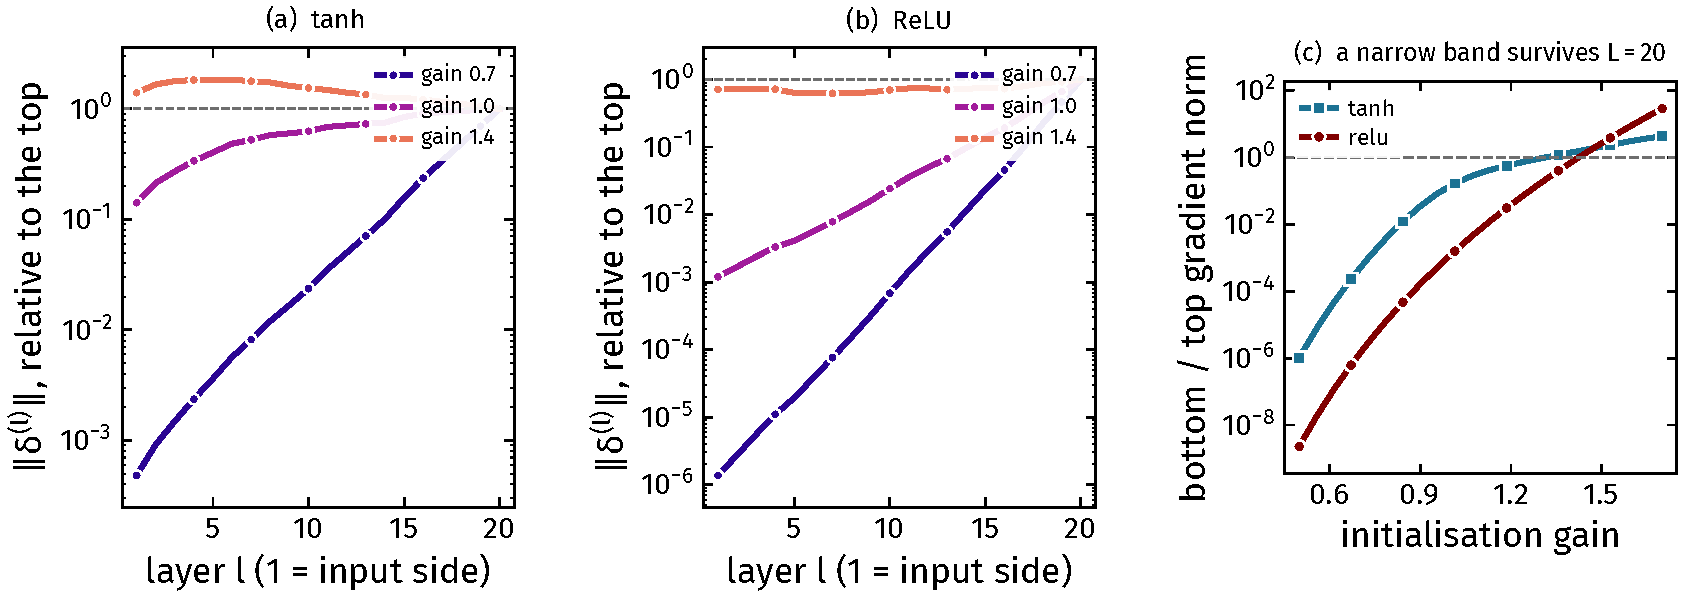
\includegraphics[height=0.485\textheight]{vanishing_exploding}
  \end{center}
  \figcap[0.96]{Norm of the backpropagated signal at each layer, relative
  to the top, for a 20-layer network. (a) $\tanh$ and (b) ReLU, at three
  initialisation gains. (c) the ratio between the bottom and top layers
  as the gain varies: only a narrow band around one survives the
  descent.}
\end{frame}

% =====================================================================
\section{Automatic Differentiation}
% =====================================================================

\begin{frame}{Three ways to differentiate a program}
  \bridge{Backpropagation was derived for one architecture. Real
  networks branch, share weights and change shape --- so we want the
  general version.}
  \vspace{0.3em}
  \centering
  \renewcommand{\arraystretch}{1.3}
  {\small
  \begin{tabular}{p{0.20\textwidth} p{0.34\textwidth}
                  p{0.34\textwidth}}
    \textbf{Method} & \textbf{How} & \textbf{Why it is not enough}\\
    \hline
    Numerical & perturb and difference
      & $O(W^{2})$, and only $8$ digits at best\\
    Symbolic & manipulate the formula
      & expression swell; needs a closed form\\
    \alert{Automatic} & apply the chain rule to the
      \alert{computational graph}
      & --- \\
    \hline
  \end{tabular}}
  \vspace{0.6em}

  {\small Automatic differentiation is \alert{exact} to machine
  precision, works on any program with branches and loops, and costs a
  constant times the function itself.}
\end{frame}

\begin{frame}{The computational graph}
  \bridge{Any program that computes $E$ is a chain --- or a DAG --- of
  elementary operations, each of which knows its own derivative.}
  \vspace{0.05em}
  \centering
  \begin{tikzpicture}[>=Stealth, line width=0.9pt, font=\small,
      x=16mm, y=11mm, scale=0.86, transform shape,
      op/.style={draw=shc, fill=shc!10, rounded corners=1.5pt,
                 minimum width=11mm, minimum height=7mm, inner sep=1pt,
                 font=\small},
      vv/.style={circle, draw=black!50, fill=black!4,
                 minimum size=9mm, inner sep=0pt, font=\small}]
    % --- forward track
    \node[vv] (x)  at (0,0) {$x$};
    \node[op] (m1) at (1,0) {$\times w$};
    \node[vv] (v1) at (2,0) {$v_1$};
    \node[op] (m2) at (3,0) {$h$};
    \node[vv] (v2) at (4,0) {$v_2$};
    \node[op] (m3) at (5,0) {$(\cdot-y)^2$};
    \node[vv] (E)  at (6,0) {$E$};
    \foreach \a/\b in {x/m1, m1/v1, v1/m2, m2/v2, v2/m3, m3/E}
      \draw[->, shc] (\a) -- (\b);
    \node[shc, font=\scriptsize] at (3,0.85) {forward: values};

    % --- backward track, on its own row so nothing overlaps
    \node[vv, draw=dpc, fill=dpc!6] (bw) at (0,-1.6) {$\bar w$};
    \node[vv, draw=dpc, fill=dpc!6] (b1) at (2,-1.6) {$\bar v_1$};
    \node[vv, draw=dpc, fill=dpc!6] (b2) at (4,-1.6) {$\bar v_2$};
    \node[vv, draw=dpc, fill=dpc!6] (bE) at (6,-1.6) {$\bar E=1$};
    \draw[->, dpc, line width=1.1pt] (bE) -- node[above,
      font=\scriptsize] {$\times\,2(v_2-y)$} (b2);
    \draw[->, dpc, line width=1.1pt] (b2) -- node[above,
      font=\scriptsize] {$\times\,h'(v_1)$} (b1);
    \draw[->, dpc, line width=1.1pt] (b1) -- node[above,
      font=\scriptsize] {$\times\,x$} (bw);
    \node[dpc, font=\scriptsize] at (3,-2.35) {backward: adjoints};

    % --- the two tracks share the same nodes
    \foreach \t/\b in {v1/b1, v2/b2, E/bE}
      \draw[mcMuted, dotted, line width=0.7pt] (\t) -- (\b);
  \end{tikzpicture}
  \vspace{0.35em}
  {\footnotesize
  \begin{itemize}\setlength{\itemsep}{0pt}
    \item Each operation contributes one \alert{local} derivative;
          nothing global is ever formed
    \item \alert{Forward mode} pushes derivatives along the top row;
          \alert{reverse mode} pulls them back along the bottom
  \end{itemize}}
\end{frame}

\begin{frame}{Forward mode}
  \vspace{0.2em}
  Carry a \alert{tangent} $\dot v = \partial v/\partial x_d$ alongside
  every value, for one chosen input $x_d$:
  \[
    v = f(u) \;\Longrightarrow\; \dot v = f'(u)\,\dot u,
    \qquad
    v = u_1 u_2 \;\Longrightarrow\; \dot v = \dot u_1 u_2 + u_1 \dot u_2
  \]
  \vfill
  {\small
  \begin{itemize}\setlength{\itemsep}{4pt}
    \item Seed $\dot x_d = 1$ and all other inputs' tangents to $0$,
          then sweep \alert{forwards} once
    \item One sweep gives $\partial v/\partial x_d$ for \alert{every}
          intermediate $v$ --- a whole column of the Jacobian
    \item Implemented neatly with \alert{dual numbers}
          $u + \dot u\,\epsilon$ where $\epsilon^{2}=0$
    \item Cost: \alert{$D$ sweeps} for $D$ inputs
  \end{itemize}}
  \fbpar{one input at a time}
        {one output at a time --- and we have only one output}
\end{frame}

\begin{frame}{Reverse mode}
  \vspace{0.05em}
  Carry an \alert{adjoint} $\bar v = \partial E/\partial v$ instead, and
  sweep the other way:
  \[
    \bar u \;=\; \sum_{v\,\in\,\mathrm{children}(u)}
    \bar v \, \frac{\partial v}{\partial u}
  \]
  \vfill
  {\small
  \begin{itemize}\setlength{\itemsep}{0pt}
    \item Seed $\bar E = 1$ and sweep \alert{backwards} once
    \item One sweep gives $\partial E/\partial v$ for \alert{every}
          node --- a whole \emph{row} of the Jacobian, which for a
          scalar $E$ is the entire gradient
    \item Needs the forward values, so they must be \alert{stored}
          on the way up
    \item Cost: \alert{$K$ sweeps} for $K$ outputs --- and $K=1$
  \end{itemize}}
  \vspace{0.05em}
  \begin{redhighlight}
    {\small \alert{Backpropagation is reverse-mode AD} on a layered
    graph: the $\delta^{(l)}_j$ are the adjoints $\bar a^{(l)}_j$.}
  \end{redhighlight}
\end{frame}

\begin{frame}{Which mode, and why}
  \bridge{The same trace, seeded from opposite ends.}
  \vspace{0.0em}
  \centering
  \begin{tikzpicture}[>=Stealth, line width=0.9pt, font=\small,
      x=15mm, y=10mm, scale=0.743, transform shape,
      vv/.style={circle, draw=black!50, fill=black!4,
                 minimum size=8.5mm, inner sep=0pt, font=\small},
      seed/.style={rounded corners=2pt, draw=accc, fill=accc!12,
                   minimum height=7mm, inner sep=3pt, font=\scriptsize}]
    % ---------- forward mode
    \node[font=\small, shc, anchor=west] at (-1.65,0.95)
      {\textbf{forward mode}};
    \node[seed] (sf) at (-1.0,0) {$\dot x_d=1$};
    \foreach \i in {0,1,2,3} \node[vv] (f\i) at (\i,0) {$v_{\i}$};
    \node[vv, draw=shc, fill=shc!8] (fE) at (4,0) {$E$};
    \draw[->, accc, line width=1.2pt] (sf) -- (f0);
    \foreach \a/\b in {f0/f1, f1/f2, f2/f3, f3/fE}
      \draw[->, shc, line width=1.2pt] (\a) -- node[above,
        font=\scriptsize, shc] {$\dot v$} (\b);
    \node[font=\scriptsize, mcMuted, anchor=west] at (4.5,0)
      {one column of $\mathbf{J}$};

    % ---------- reverse mode
    \node[font=\small, dpc, anchor=west] at (-1.65,-1.55)
      {\textbf{reverse mode}};
    \foreach \i in {0,1,2,3} \node[vv] (r\i) at (\i,-2.5) {$v_{\i}$};
    \node[vv, draw=dpc, fill=dpc!8] (rE) at (4,-2.5) {$E$};
    \node[seed] (sr) at (5.35,-2.5) {$\bar E=1$};
    \draw[->, accc, line width=1.2pt] (sr) -- (rE);
    \foreach \a/\b in {rE/r3, r3/r2, r2/r1, r1/r0}
      \draw[->, dpc, line width=1.2pt] (\a) -- node[above,
        font=\scriptsize, dpc] {$\bar v$} (\b);
    \node[font=\scriptsize, mcMuted, anchor=east] at (-0.6,-2.5)
      {one \emph{row} of $\mathbf{J}$};
  \end{tikzpicture}
  \vspace{-0.05em}
  {\footnotesize
  \begin{itemize}\setlength{\itemsep}{0pt}
    \item Forward mode needs \alert{one sweep per input}: $D$ of them.
          Reverse mode needs \alert{one per output}: $K$ of them
    \item Training has $D=W$ inputs and $K=1$ output, so reverse mode
          wins by a factor of $W$ --- millions to one
    \item The price is that reverse mode must \alert{store} the forward
          values before it can use them
  \end{itemize}}
\end{frame}

\begin{frame}{The cheap gradient principle}
  \vspace{0.3em}
  \begin{theorem}[Baur \& Strassen, 1983]
    {\small Let $f:\mathbb{R}^{D}\to\mathbb{R}$ be computed by a
    straight-line program of $C$ arithmetic operations. Then the full
    gradient $\nabla f$ can be computed in $O(C)$ operations ---
    in fact at most about $4C$, \alert{independent of $D$}.}
  \end{theorem}
  \vspace{0.5em}
  {\small
  \begin{itemize}\setlength{\itemsep}{4pt}
    \item A gradient with a million components costs no more than about
          four function evaluations
    \item The $O(W)$ cost of backpropagation is a \alert{special case}
          of this, not a property of neural networks
    \item The price is \alert{memory}: reverse mode must retain the
          forward values, so storage grows with the graph
  \end{itemize}}
\end{frame}

\begin{frame}{What it costs in memory, and how to pay less}
  \vspace{0.3em}
  {\small
  \begin{itemize}\setlength{\itemsep}{5pt}
    \item The backward pass needs every stored $\mathbf{a}^{(l)}$ and
          $\mathbf{z}^{(l)}$: memory grows \alert{linearly with depth}
          and with the batch size
    \item \alert{Gradient checkpointing}: keep only every
          $\sqrt{L}$-th layer's activations and recompute the rest
          during the backward pass --- memory $O(\sqrt{L})$ for about
          one extra forward pass
    \item \alert{Reversible layers} go further: reconstruct
          $\mathbf{z}^{(l-1)}$ from $\mathbf{z}^{(l)}$ and store
          nothing
    \item This trade --- recompute versus retain --- is why very deep
          models are trainable on finite hardware
  \end{itemize}}
  \fbpar{cheap in time, expensive in memory}
        {checkpointing trades one back for the other}
\end{frame}

\begin{frame}{How the frameworks do it}
  \vspace{0.3em}
  {\small
  \begin{itemize}\setlength{\itemsep}{4pt}
    \item \alert{Tape-based (PyTorch).} Every operation on a tracked
          tensor appends a node recording its inputs and its local
          derivative. Calling \texttt{backward()} walks the tape in
          reverse. The graph is built afresh each iteration, so
          branches and loops are free.
    \item \alert{Trace-and-transform (JAX).} The function is traced
          once into a graph, then a program transformation
          (\texttt{grad}) produces a new program computing the
          gradient, which is then compiled.
    \item Both are reverse-mode AD. Neither contains anything specific
          to neural networks --- a network is just one program among
          many.
  \end{itemize}}
  \vspace{0.3em}
  \begin{redhighlight}
    {\small You will never implement backpropagation. You will
    regularly \alert{debug} it --- which needs the equations in \S4.}
  \end{redhighlight}
\end{frame}

% =====================================================================
\section{Putting It Together}
% =====================================================================

\begin{frame}{One training step, end to end}
  \vspace{0.3em}
  \centering
  \begin{tikzpicture}[>=Stealth, line width=0.9pt, font=\small,
      scale=0.86, transform shape,
      b/.style={rounded corners=3pt, draw=shc, fill=shc!7,
                align=center, minimum height=0.95cm,
                inner xsep=4pt, font=\footnotesize},
      lbl/.style={font=\scriptsize\itshape, mcMuted}]
    \node[b] (a) {sample a\\mini-batch};
    \node[b, right=5mm of a] (b) {forward pass\\store $\mathbf{a},\mathbf{z}$};
    \node[b, right=5mm of b] (c) {error\\$E(\mathbf{w})$};
    \node[b, right=5mm of c, draw=dpc, fill=dpc!7] (d)
      {$\bm\delta^{(L+1)}$\\$=\hat{\mathbf{y}}-\mathbf{y}$};
    \node[b, right=5mm of d, draw=dpc, fill=dpc!7] (e)
      {backward pass\\$\bm\delta^{(l)}$};
    \node[b, right=5mm of e, draw=dpc, fill=dpc!7] (f)
      {$\nabla E=\bm\delta\mathbf{z}^{\top}$};
    \node[b, below=6mm of f] (g) {update\\$\mathbf{w}\!\leftarrow\!
      \mathbf{w}-\eta\nabla E$};
    \draw[->] (a)--(b); \draw[->] (b)--(c); \draw[->] (c)--(d);
    \draw[->, dpc] (d)--(e); \draw[->, dpc] (e)--(f); \draw[->] (f)--(g);
    \draw[->] (g) -| (a);
    \node[lbl, below=1mm of b] {\S2--3};
    \node[lbl, below=1mm of e] {\S4--5};
  \end{tikzpicture}
  \vspace{0.6em}
  {\small
  \begin{itemize}\setlength{\itemsep}{2pt}
    \item Everything in maroon is one call to \texttt{backward()}
    \item The update rule itself --- how to choose $\eta$, and what to
          do instead of plain descent --- is \alert{Class 13}
  \end{itemize}}
\end{frame}

\begin{frame}{Takeaways}
  \vspace{-0.05em}
  {\footnotesize
  \begin{enumerate}\setlength{\itemsep}{0pt}
    \item An activation is chosen for its \alert{derivative}: the
          logistic caps $h'$ at $\tfrac14$; ReLU does not saturate but
          its units can \alert{die permanently}
    \item Pairing an output activation with the matching error function
          is the \alert{canonical link}, and it makes
          $\partial E/\partial a = \hat y - y$ --- one theorem behind
          the three cases of Class 6
    \item Error functions extend past those three:
          \alert{heteroscedastic} outputs predict $\sigma(x)$,
          \alert{mixture density} outputs keep multi-valued answers
          that squared error would average away
    \item \alert{Backpropagation} splits every derivative as
          $\delta^{(l)}_j z^{(l-1)}_i$ and gets all $W$ of them in
          $O(W)$ --- against $O(W^{2})$ for finite differences
    \item It is \alert{reverse-mode automatic differentiation} on the
          computational graph, and by Baur--Strassen the gradient costs
          a small constant times the function, at the price of memory
  \end{enumerate}}
  \vspace{0.05em}
  \begin{redhighlight}
    {\footnotesize Class 13: we can compute $\nabla E$ cheaply and
    exactly. Next, what to \alert{do} with it --- gradient descent and
    its modern variants.}
  \end{redhighlight}
\end{frame}

\begin{frame}{References}
  \scriptsize
  \begin{itemize}\setlength{\itemsep}{2pt}
    \item C.~M.~Bishop \& H.~Bishop. \textit{Deep Learning: Foundations
          and Concepts.} Springer, 2024. \S6.2--6.3 (activation
          functions), \S6.4 (error functions and the canonical link),
          \S6.5 (mixture density networks), Ch.~8 (backpropagation,
          \S8.1; automatic differentiation, \S8.2).
    \item S.~J.~D.~Prince. \textit{Understanding Deep Learning.}
          MIT Press, 2023. Ch.~5 (loss functions, including
          heteroscedastic and mixture models), Ch.~7 (gradients,
          backpropagation, initialisation and the exploding-gradient
          problem).
    \item W.~Baur \& V.~Strassen, \textit{Theoretical Computer Science}
          22:317 (1983) --- the complexity of partial derivatives:
          the ``cheap gradient'' result.
    \item D.~Rumelhart, G.~Hinton \& R.~Williams, \textit{Nature}
          323:533 (1986) --- learning representations by
          back-propagating errors.
    \item A.~Baydin, B.~Pearlmutter, A.~Radul \& J.~Siskind,
          \textit{JMLR} 18:153 (2018) --- automatic differentiation in
          machine learning: a survey.
    \item Plots generated by \texttt{src/build\_all.py}; one module per
          figure under \texttt{src/figures/}.
  \end{itemize}
\end{frame}

\begin{frame}[standout]
  Questions?
\end{frame}

\end{document}
